\section{Clumping Factors and the Photon Budget for Reionization}
\label{sec:ClumpingFactors}



\subsection{Clumping Factor Analysis of Madau}
\label{Madau}
In this section we begin our examination of Equation \eqref{eq:ndot} from \cite{MadauEtAl1999} as an accurate predictor of when reionization completes, focusing on the clumping factor. While  it is true that the Madau-type analysis was not designed to predict the precise redshift for reionization completion, only the ionization rate density needed to maintain the IGM in an ionized state after reionization has completed, it is effectively being used in this way when it is applied to galaxy populations at increasingly higher redshifts $z=6-7$  (cf. \cite{FanEtAl2006, RobertsonEtAl2013}).
Our methodology is the following. The simulation supplies $\dot{N}_{sim}(z)$ ionizing photons, which increases with decreasing redshift because the SFRD increases with decreasing redshift.  Equation \eqref{eq:ndot} poses a minimum requirement on the ionizing emissivity to maintain the IGM in an ionized state at given redshift z. This requirement decreases with decreasing redshift due to the strong z dependence.  We look to see if the box becomes fully ionized when these two curves cross; i.e., when $\dot{N}_{sim} \geq \dot{\mathcal{N}}_{ion} $. In subsequent sections we do this for more recent definitions of the clumping factor that have been introduced by various authors, in roughly chronological order. 

%\subsubsection{Original Methods}
%\label{OriginalMethods}

The way the clumping factor is introduced and used, is to estimate the amount of recombination that radiation has to overcome, in order to keep the universe ionized \citep{GnedinOstriker1997,ValageasSilk1999,MadauEtAl1999,FanEtAl2006}.  In a homogeneous universe, the hydrogen recombination rate is also homogeneous, and is a simple function of the mean density, ionization fraction, and temperature. The clumping factor is a correction factor to account for density inhomogeneities induced by structure formation, although in principle inhomogeneties in ionization fraction and temperature are also important.   
%In its original definition, the clumping factor is defined when only hydrogen information is available.  Therefore, when the universe is 100\% ionized, the free %electron number density equals that of the hydrogen number density denoted by $n_\mathrm{H\,II}$, multiplied by $(1+2\chi)$, where $\chi$ is the cosmic fraction of helium to hydrogen.  
The most common definition for the clumping factor is:
\begin{equation}
	C=\frac{\langle n_\mathrm{H\,II}^2 \rangle}{\langle n_\mathrm{H\,II} \rangle^2}
	\label{eq:clumpingfactor}
\end{equation}
Where the $\langle\rangle$ brackets denotes an average over the simulation volume. To see where this comes from lets look at the change of $n_\mathrm{H\,II}$ with respect to time due to recombinations:
%Paraphrasing the original authors, if we only consider the non-expanding cosmological box, 
%To see where this comes from look at the change of $n_\mathrm{H\,II}$ with respect to time of 
% recombination $t_{rec}$, using the recombination portion of Equation \eqref{eq:chemical_ionization},
\begin{align}
	\label{eq:recombtime}
	\frac{\partial n_\mathrm{H\,II}}{\partial t} 
&= -n_\mathrm{e} n_\mathrm{H\,II}\alpha_B(T)\notag\\
	\frac{\partial n_\mathrm{H\,II}}{n_\mathrm{H\,II}} 
&= -\partial t n_\mathrm{e}\alpha_B(T)\notag\\
	\int^{n_f}_{n_i}\frac{\partial n_\mathrm{H\,II}}{n_\mathrm{H\,II}} 
&= -\int^{t_f}_{t_i}\partial t n_\mathrm{e}\alpha_B(T)\notag\\
	ln\left(\frac{n_f}{n_i}\right) 
&= -(t_f-t_i)n_\mathrm{e}\alpha_B(T), \notag\\
	\frac{n_f}{n_i} 
&= exp(-t_{rec}n_\mathrm{e}\alpha_B)
\end{align}
In the last step, we have set $(t_f-t_i)$ to be $t_{rec}$.  This leads to 
\begin{equation}
    t_{rec} = [n_\mathrm{e}\alpha_B(T)]^{-1}
    \label{recombtime}
\end{equation}
being the characteristic time when the fraction $n_f/n_i =  1/e$.  Using this expression for the recombination time, one can rewrite the right hand side of the equation as
\begin{align}
	\label{eq:trec}
	\frac{\partial n_\mathrm{H\,II}}{\partial t} 
&= - n_\mathrm{H\,II}n_\mathrm{e}\alpha_B(T) = - n_\mathrm{H\,II} / t_{rec}\notag\\
&= - n_\mathrm{H\,II} (1+2\chi) n_\mathrm{H\,II} \alpha_B(T) \notag\\
&= - n_\mathrm{H\,II}^2 (1+2\chi) \alpha_B(T) \notag\\
\end{align}
where in the last two steps, following \cite{MadauEtAl1999}, we replace $n_\mathrm{e}$ with $(1+2\chi)n_\mathrm{H\,II}$ assuming helium is fully ionized. Here $\chi$ is the cosmic fraction of helium. Taking the volume average we have:
\begin{align}
\label{eq:trecpart2}
	\langle \frac{\partial n_\mathrm{H\,II}}{\partial t} \rangle
&= - \langle n_\mathrm{H\,II}^2 (1+2\chi) \alpha_B(T) \rangle \notag\\
&= - \langle n_\mathrm{H\,II}^2 \rangle (1+2\chi) \alpha_B \notag\\
&= - \langle n_\mathrm{H\,II} \rangle^2 (1+2\chi) \alpha_B C\notag\\
&= - \langle n_\mathrm{H\,II} \rangle /\bar{t}_{rec}
\end{align}
%When all the helium is ionized, one is justified to replace $n_\mathrm{e}$ by %$(1+2\chi)n_\mathrm{H\,II}$.  
In the above we have made the oft-used assumption of a uniform IGM temperature of $10^4$K, making the Case B recombination coefficient, $\alpha_B$ a constant.  Note this is not physically justified, but since the temperature of the IGM is not well determined observationally, it is a useful approximation, and one that is embedded in Equation \eqref{eq:ndot}. With this simplifying assumption, when taking the volume average on both sides of the equation, we may rewrite the result in the same form as the first line in Equation \eqref{eq:trec}.  Therefore, the effective recombination time can be written as 
\begin{equation}
	\bar{t}_{rec} = t_\mathrm{Madau} \equiv [(1+2\chi)\langle n_\mathrm{H\,II} \rangle \alpha_B C]^{-1}
	\label{eq:tmadau}
\end{equation}
%We are hesitant to label the recombination time $t_\mathrm{Madau}$ as a mean quantity here, %as oppose to \cite{MadauEtAl1999}, which we will discuss in more detail in \S\ref{Discussion}.
This expression is the same as Equation (20) of \cite{MadauEtAl1999} if we substitute $\langle n_\mathrm{H\,II} \rangle$ for $\bar{n}_\mathrm{H}$. In the case of a fully ionized universe these two quantities are equivalent. We note that $t_\mathrm{Madau}$ is not at all the volume average of $t_{rec}$ but is $\langle t_{rec}^{-1} \rangle ^{-1}C^{-1}$, which weights regions
with the {\em shortest} recombination times; i.e. regions at the mean density and above. If we now make the 
{\em ansatz} $\dot{\mathcal{N}}_{ion} \times \bar{t}_{rec} = \bar{n}_\mathrm{H}(0)$, we may derive Equation (26) in \cite{MadauEtAl1999}, updated by \cite{FanEtAl2006}, repeated here for convenience:
%If the clumping factor is calculated from an accurate simulation, then the clumping factor can 
%be used in the above work's Equation (24) in semi-analytical models to predict the ionization 
%rate.  One will arrive at the equation
\begin{equation}
	\label{eq:updatedNdot}
	\dot{\mathcal{N}}(z)=10^{51.2}s^{-1}Mpc^{-3}\left(\frac{C}{30}\right)\left(\frac{\Omega_\mathrm{b} h^2}{0.02}\right)^{2}\left(\frac{1+z}{6}\right)^{3}.
\end{equation}

%and updated in \citep{FanEtAl2006} with appropriate assumptions.  
This equation gives an estimate of the ionizing photon production rate density (in units of s$^{-1}$Mpc$^{-3}$comoving) that is needed to balance the recombination rate density (the right-hand-side of Equation \eqref{eq:updatedNdot}) in a completely ionized universe.  Values for $C$ ranging $\sim$10-30 are often quoted from earlier hydrodynamical simulations such as \cite{GnedinOstriker1997}, and $\sim 3$ for more recent work following \cite{PawlikEtAl2009, RaicevicTheuns2011, ShullEtAl2012, FinlatorEtAl2012} and the methods there.
\begin{figure}
	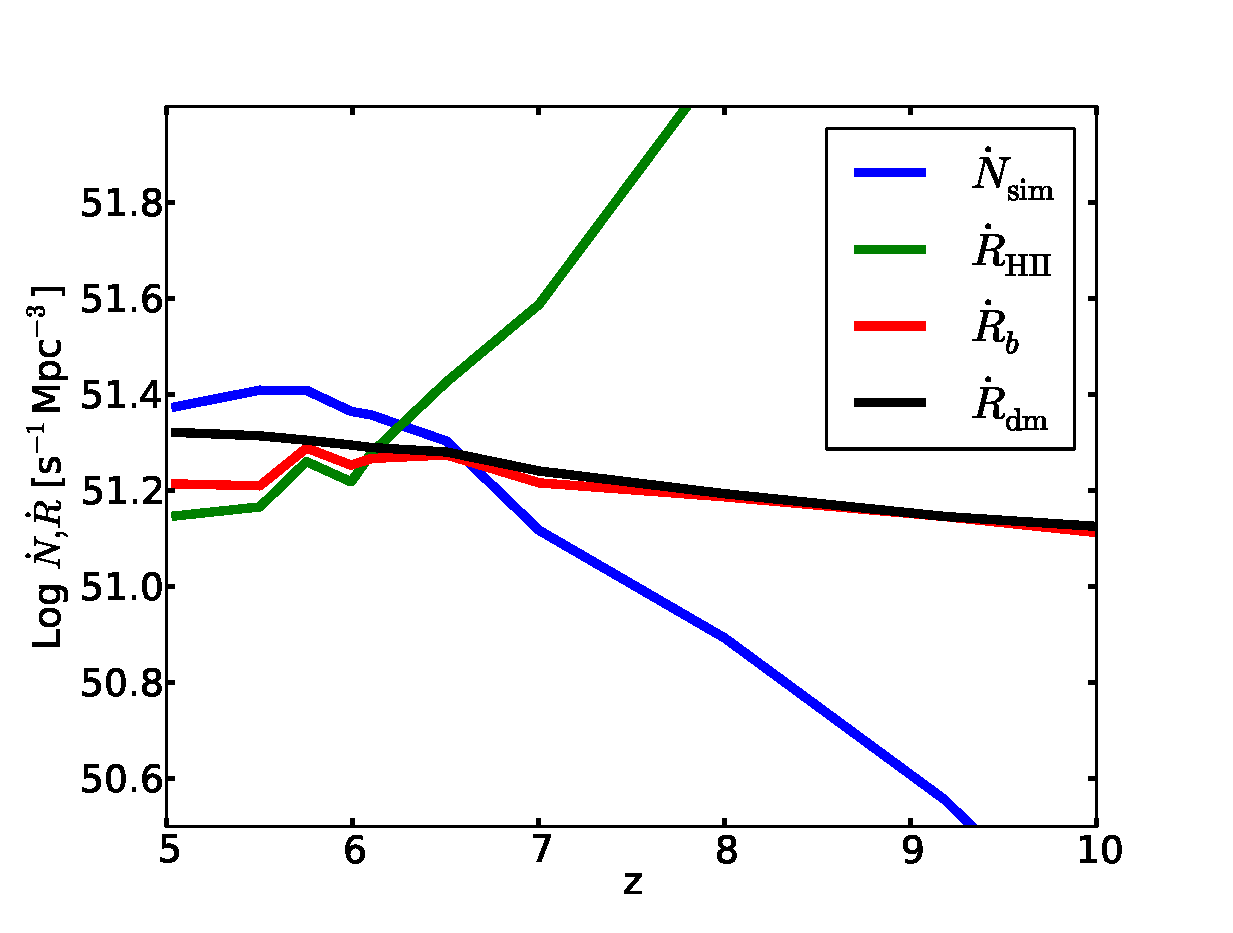
\includegraphics[width=0.5\textwidth]{unthresholded.eps}
 %       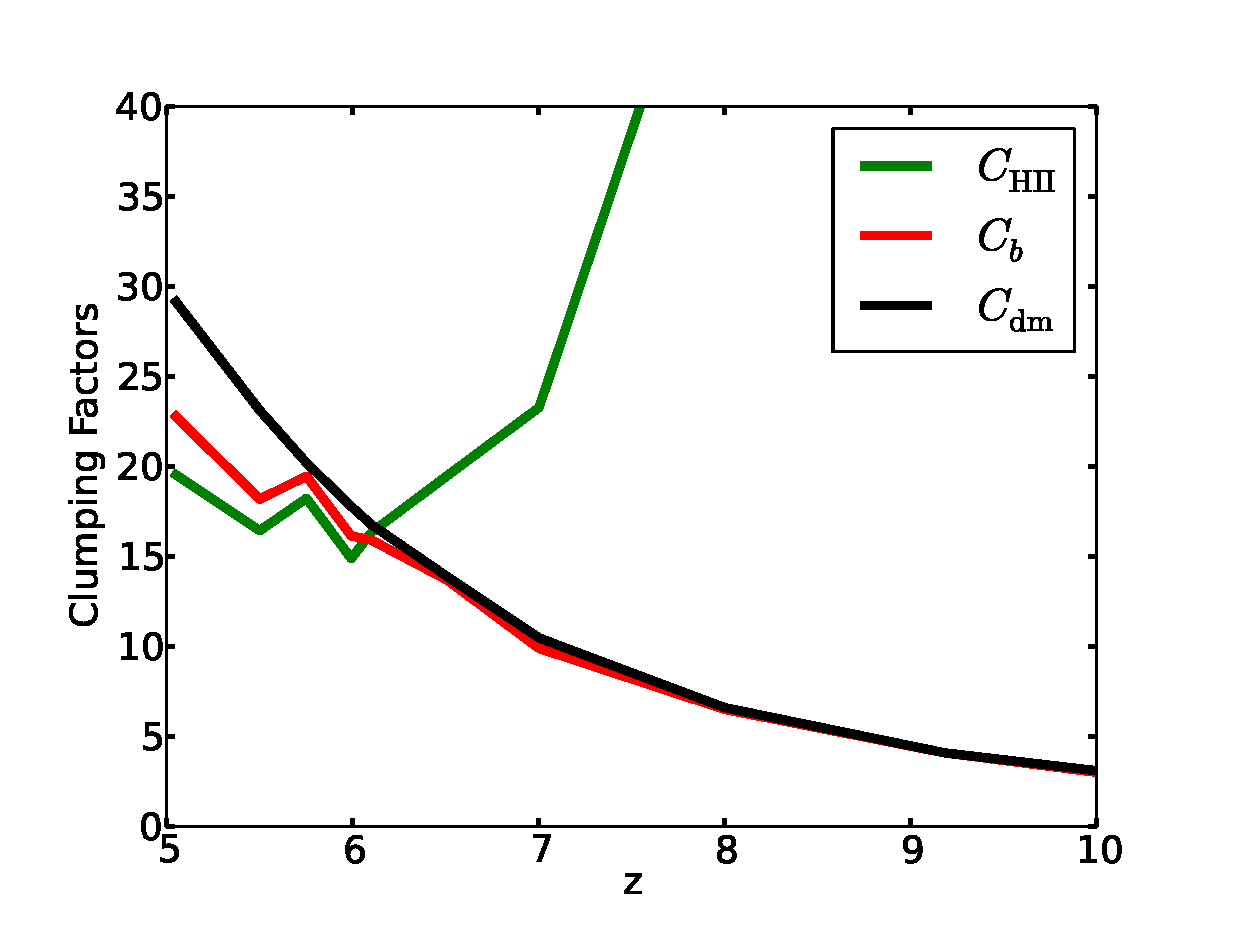
\includegraphics[width=0.5\textwidth]{unthreshclumping.eps}
	\caption{Ionizing photon production rate density and various estimates of the recombination rate density versus redshift. The blue curve labeled ``$\dot{N}_{sim}$'' is the measured photon production rate density averaged over the entire simulation volume. The green curve labeled ``$\dot{R}_\mathrm{H\,II}$'' is the recombination rate density estimate from using the clumping factor calculated with Equation \eqref{eq:clumpingfactor} substituted in Equation \eqref{eq:updatedNdot}. The red curve labeled ``$\dot{R}_b$'' is Equation \eqref{eq:updatedNdot} evaluated using a clumping factor calculated from the baryon density. The black curve labeled ``$\dot{R}_\mathrm{dm}$'' is using a clumping factor calculated with dark matter density.}
	\label{unthresholded}
\end{figure}

\begin{figure}
	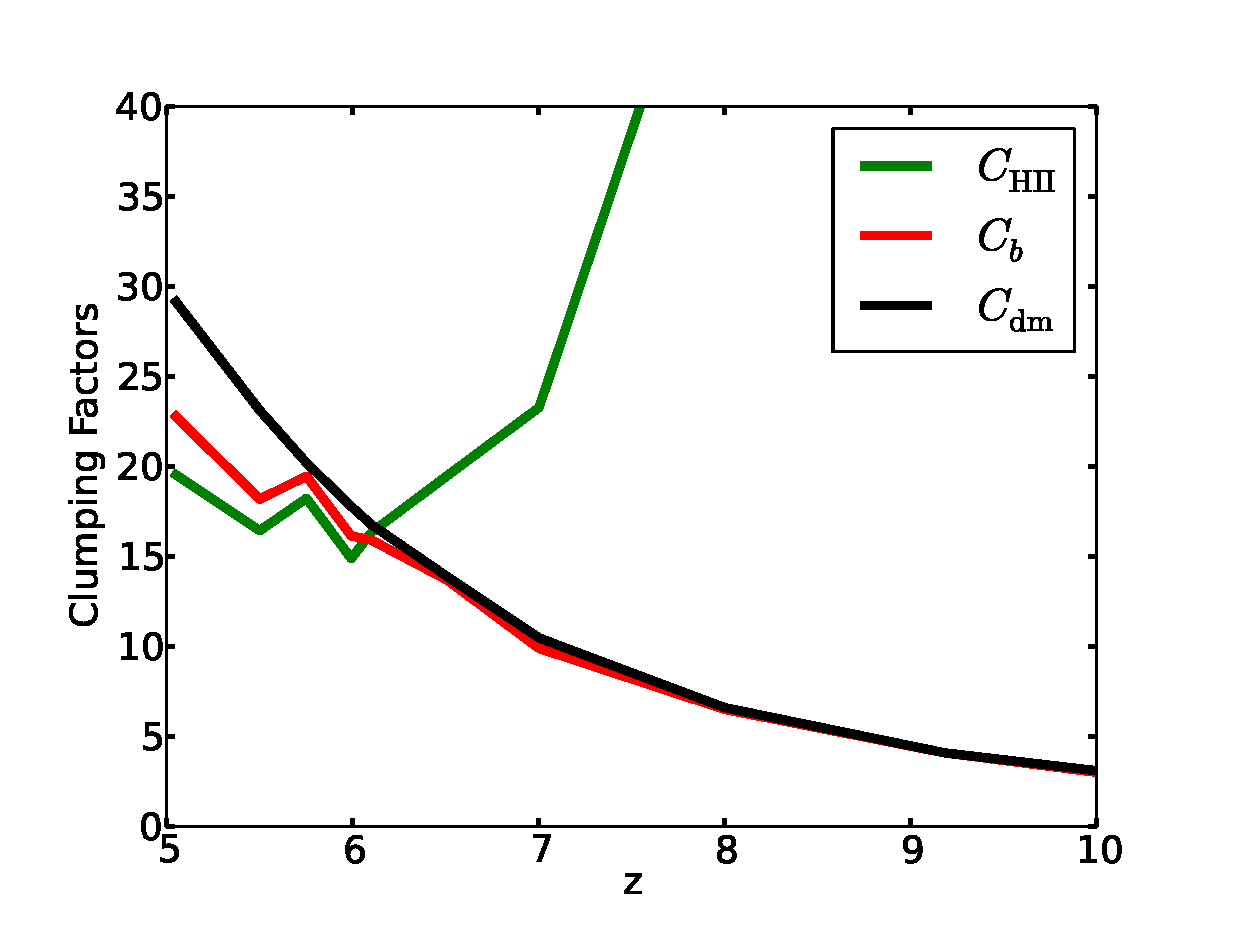
\includegraphics[width=0.5\textwidth]{unthreshclumping.eps}
	\caption{Unthresholded clumping factors used in Fig. \ref{unthresholded}. $C_{HII}, C_b, C_{dm}$ are calculated from the unthresholded H \footnotesize{II}, baryon, and dark matter densities, respectively.}
	\label{unthreshclumping}
\end{figure}

We follow these earlier studies using our own simulation data.  In Figure \ref{unthresholded} we plot the ionizing photon production rate density and recombination rate density from our fiducial simulation.  The curve in blue labeled $\dot{N}_{sim}$ is the photon production rate density from the simulation, calculated using a time average of the volume integrated ionizing emissivity $\eta$ (Equation \eqref{eq:emissivity}) divided by the average energy per photon which we obtain directly from the SED.  The other three curves plot Equation \eqref{eq:updatedNdot} for three methods for calculating $C$: green uses the H {\footnotesize II} density directly (Equation \eqref{eq:clumpingfactor}); red uses the baryon density $C=\langle \rho^2_b \rangle / \langle \rho_b \rangle^2$; and black uses the dark matter density $C=\langle \rho^2_{dm} \rangle / \langle \rho_{dm} \rangle^2$. In all cases no thresholding is being applied (the effect of threholding is examined in the next section); the averages are done over every cell in the simulation including those inside the virial radii of galaxies. The H {\footnotesize II} curve drops sharply with decreasing redshift because $C$ is large when the H {\footnotesize II} distribution is patchy. The baryon and dark matter curves track one another for $z > 6$ because the clumping factors are nearly the same, but begin to separate after overlap as the baryon clumping factor drops due to Jeans smoothing.  

Where the ionization and recombination rate density lines cross is roughly when we expect the universe to become highly ionized.
If we define the end of the EoR as when 99.9\% of the volume has  reached the Well Ionized level, then our simulation reaches that point around $z\sim5.8$ according to Figure \ref{linearIonized}.  The $\dot{N}_{sim}$ curve crosses the $\dot{R}_\mathrm{H\,II}$ curve at $z\sim6.2$. This is somewhat reassuring since we are counting every ionizing photon emitted and every recombination, at lease insofar as Equation \eqref{eq:updatedNdot} provides a good estimate of that. The recombination rate density curves using clumping factors computed from the baryon and dark matter densities curves cross the $\dot{N}_{sim}$ curve at a somewhat higher redshift of $z \approx 6.6$. By following the original methodology of using the clumping factor to estimate recombinations, we find that the clumping factor calculated with the H {\footnotesize II} density field to be the closest predictor for the end of EoR in our simulation. 

The photon budget that enabled us to reach different levels of ionization is plotted in Figure \ref{unthreshphotonbudget}.  
Here we plot the evolution of the ionized volume fraction versus $\gamma_{ion}/H=\int dt \dot{N}_{sim} / \bar{n}_\mathrm{H}(0)$. So, for the same definition for the end of EoR, we see that we need $\sim$4 photons per hydrogen atom to  achieve. This cannot be considered a converged result because this estimate includes the dense gas inside galaxies, which is not well resolved in our simulation. Even though a small fraction of the baryons reside inside galaxies, due to the short recombination time many ionizing photons are required to keep the gas ionized.  Since we have not resolved the internal structure of galaxies, and higher resolution would likely result in higher density gas, we must consider $\gamma_{ion}/H=4$ a lower bound. We eliminate this issue in the next subsection by excluding the dense gas in halos from the calculation. 
%By the same logic, as the definition of EoR changes, so will the photon per hydrogen number.

\begin{figure}
	\includegraphics[width=0.5\textwidth]{unthresh_photon_per_H.eps}
	\caption{Ionized volume fraction as a function of the number of ionizing photons emitted per H atom averaged over the entire simulation volume (including inside halos) for three different ionization levels: $f_i \geq 0.1$ (blue line);  $f_i \geq 0.999$ (green line); $f_i \geq 0.99999$ (red line). Compare with Fig. \ref{threshphotonbudget} which excludes gas inside halos.}
	\label{unthreshphotonbudget}
\end{figure}

%\subsubsection{Investigating Thresholding Method}
%\label{InvestigatingThresholdingMethod}
\subsection{Quantitative Analysis of Recombinations}

As the clumping factor method grew in popularity, various authors have applied thresholds of one form or another to improve upon its accuracy in predicting the recombination rate density needed to maintain an ionized universe. When thresholds are applied, parts of the volume are excluded from the photon counting analysis.   \cite{PawlikEtAl2009, RaicevicTheuns2011} and others, limit the calculation of the clumping factor to the low density IGM by using $\Delta_b$ thresholds, usually set at 100.  They threshold out gas in virialized halos and the self-shielded collapsed objects, because radiation does not penetrate these objects, or they recombine too fast, which leaves them neutral and not contributing to recombinations in the IGM. More recently \cite{ShullEtAl2012} has also thresholded out void regions ($\Delta_b < 1$), arguing that they do not contribute appreciably to the total recombinations due to their long recombination times. 

To investigate the contribution of gas of different density to the total recombination rate density, we plot in Figure \ref{recomb}, three quantities dealing with recombinations in our simulation.  In the left column we have a 2D distribution plot of recombination rate density $\dot{R} = n_\mathrm{H\,II}n_e\alpha_B(T)$ divided by ionization rate density $\Gamma_\mathrm{H\,I}^{ph}n_\mathrm{H\,I}$ versus baryon overdensity $\Delta_b$, where  
\begin{align}
  \label{eq:photoionization}
  \Gamma_\mathrm{H\,I}^{ph} &= \frac{c E}{h} \left[\int_{\nu_\mathrm{H\,I}}^{\infty}
    \frac{\sigma_\mathrm{H\,I}(\nu) \chi_E(\nu)}{\nu}\,\mathrm d\nu \right]  \bigg /
  \left[\int_{\nu_\mathrm{H\,I}}^{\infty} \chi_E(\nu)\,\mathrm d\nu\right].
\end{align}
Here, $\sigma_\mathrm{H\,I}(\nu)$ and $\nu_\mathrm{H\,I}$ are the ionization cross section and ionization threshold for H {\footnotesize I}, respectively, and 
$h$ is Planck's constant (Paper I). In the middle column we plot the relative bin contribution to the total recombination rate density versus $\Delta_b$.  We draw vertical lines at $\Delta_b$=1 and 100, and in the legend box calculate the cumulative contribution to total reionizations to those thresholds.  In the right column, we plot the cell recombination time divided by the Hubble time versus $\Delta_b$.  All three columns evolve with descreasing redshift from top to bottom.

% ZahnEtAl2009 bubble threshold at x=0.9, ionized is when photon number > hydrogen number
% ShinEtAl2008 ionized when x>0.5

%\begin{figure*}[p]
%	\includegraphics[width=1.0\textwidth]{recomb.png}
%	\caption{Plot of recombination information.  Left column is a 2D distribution of recombination rate %density divide by ionization rate density versus over density.  Middle column is plot relative bin %contribution to the total recombination rate density versus over density bins.  The lines show the %cumulative of all previous bins.  Blue line is at $\Delta_b$=100, red line is at $\Delta_b$=1.  Right %column is plot of recombination time divide by Hubble time versus over density.  All three columns %evolve with descreasing redshift from top to bottom.}
%	\label{recomb}
%\end{figure*}

\begin{figure*}[!tp]
     \begin{minipage}[h]{0.33\linewidth}
        \centering
        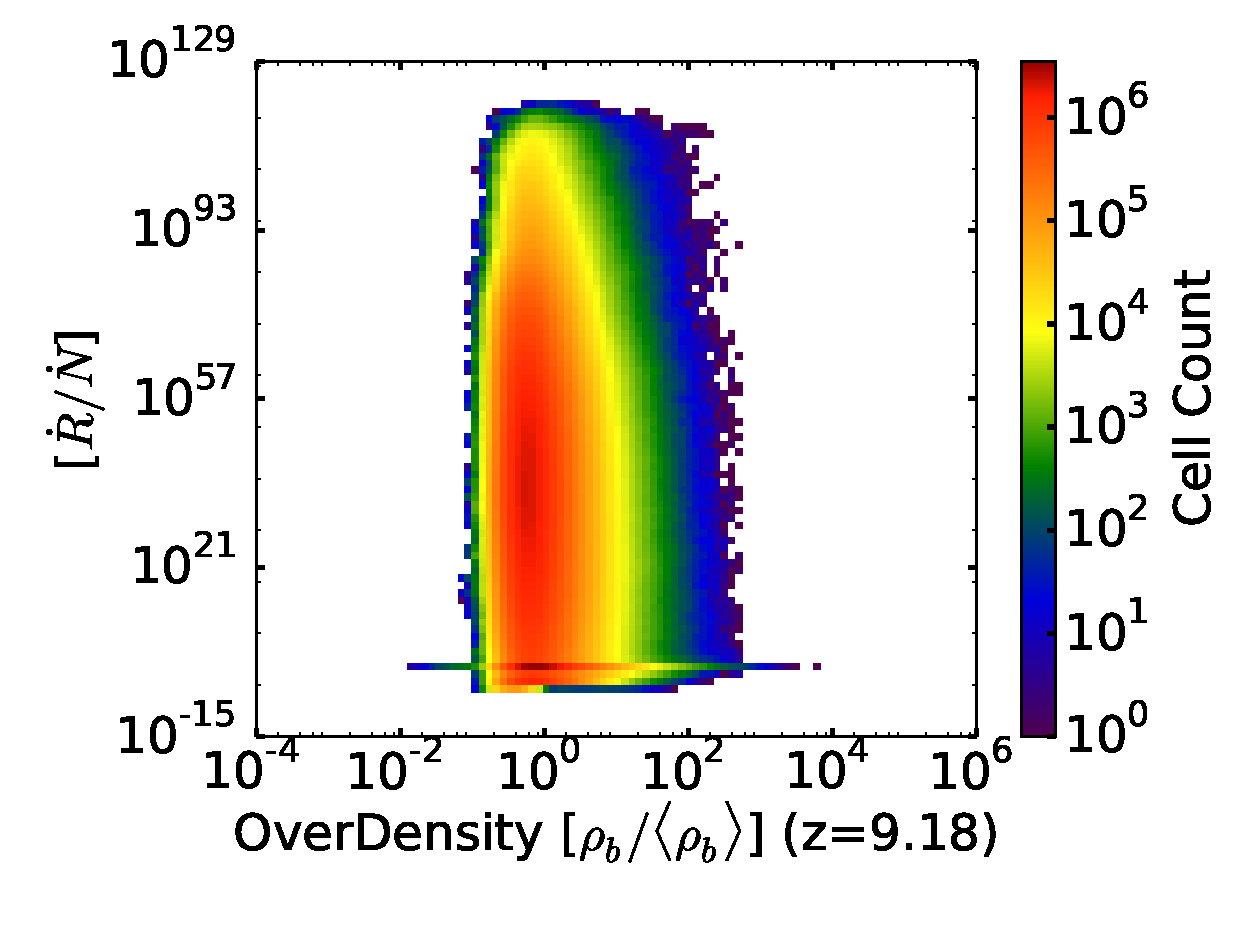
\includegraphics[trim = 5mm 8mm 0mm 0mm, clip, width=1.0\textwidth]{1_1_HD4050OverDensityRecombIonFrac.eps}
     \end{minipage}
\hspace*{-2.00mm}
    \begin{minipage}[h]{0.33\linewidth}
       \centering
       \includegraphics[trim = 5mm 8mm 0mm 0mm, clip, width=1.0\textwidth]{1_2_HD4050_recomb_contrib_v_OD.eps}
     \end{minipage}
\hspace*{-4.00mm}
    \begin{minipage}[h]{0.33\linewidth}
       \centering
       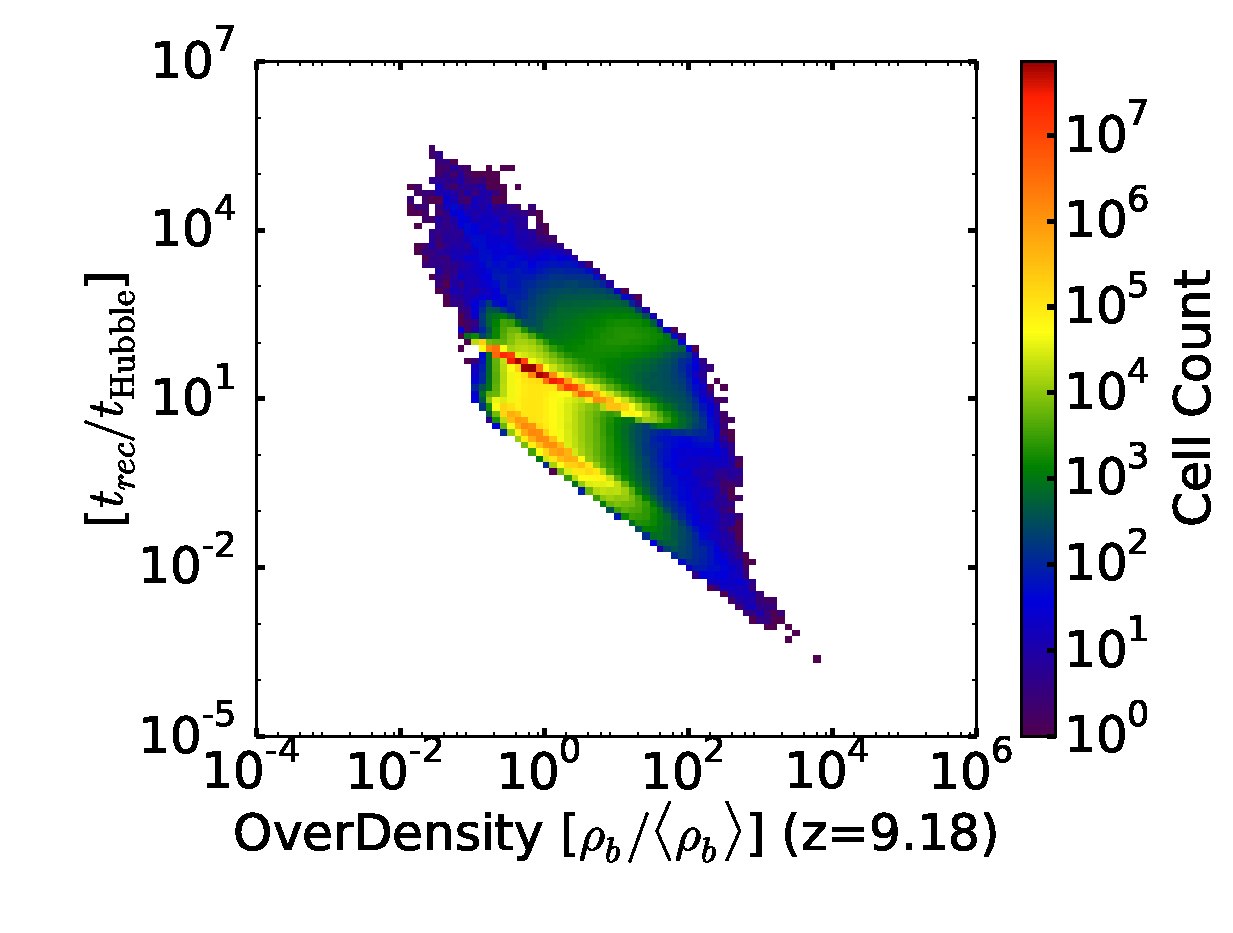
\includegraphics[trim = 5mm 8mm 0mm 0mm, clip, width=1.0\textwidth]{1_3_HD4050OverDensityRecombHubbleTime.eps}
    \end{minipage}
\\
     \begin{minipage}[h]{0.33\linewidth}
        \centering
        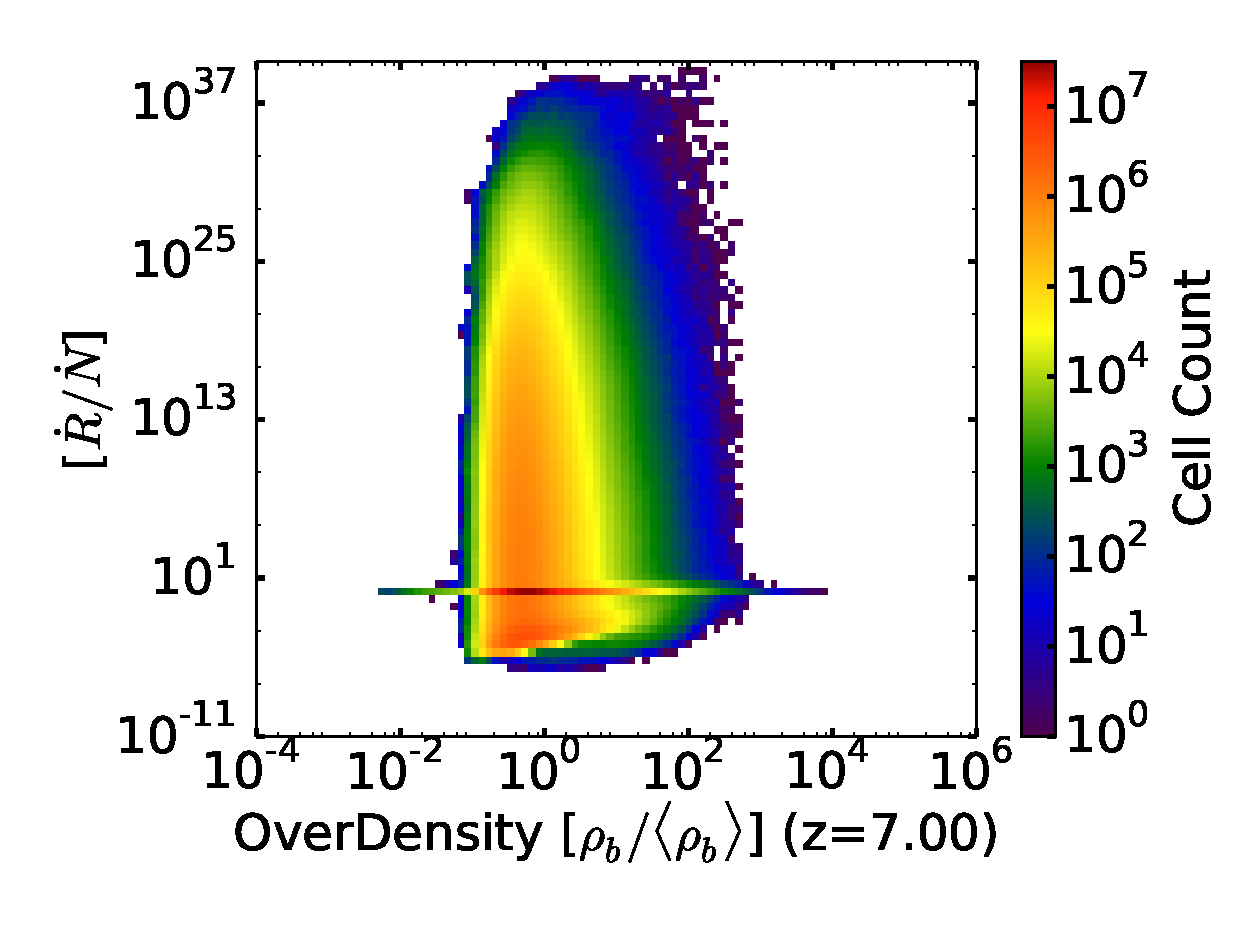
\includegraphics[trim = 5mm 8mm 0mm 0mm, clip, width=1.0\textwidth]{2_1_HD7900OverDensityRecombIonFrac.eps}
     \end{minipage}
\hspace*{-2.00mm}
    \begin{minipage}[h]{0.33\linewidth}
       \centering
       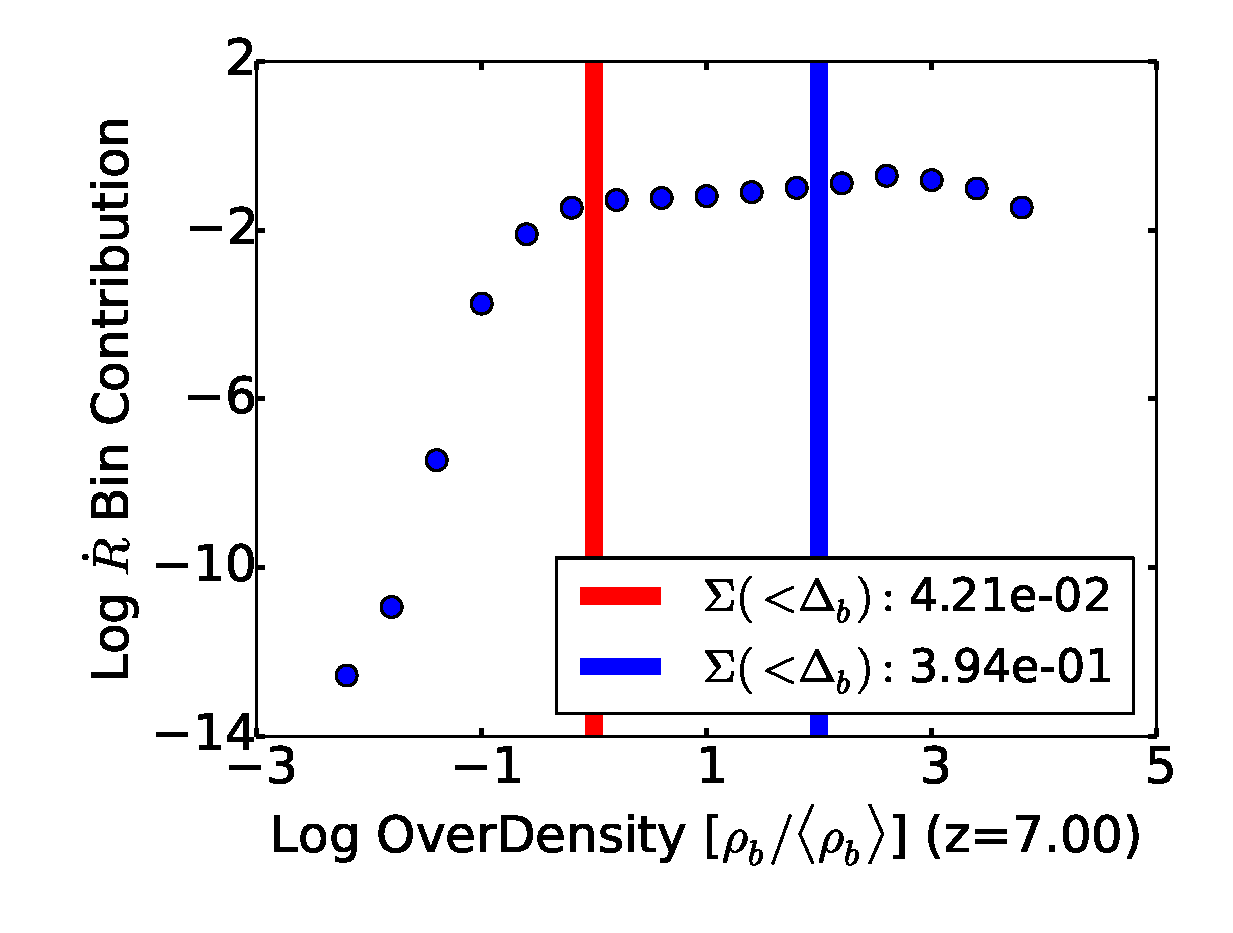
\includegraphics[trim = 5mm 8mm 0mm 0mm, clip, width=1.0\textwidth]{2_2_HD7900_recomb_contrib_v_OD.eps}
     \end{minipage}
\hspace*{-4.00mm}
    \begin{minipage}[h]{0.33\linewidth}
       \centering
       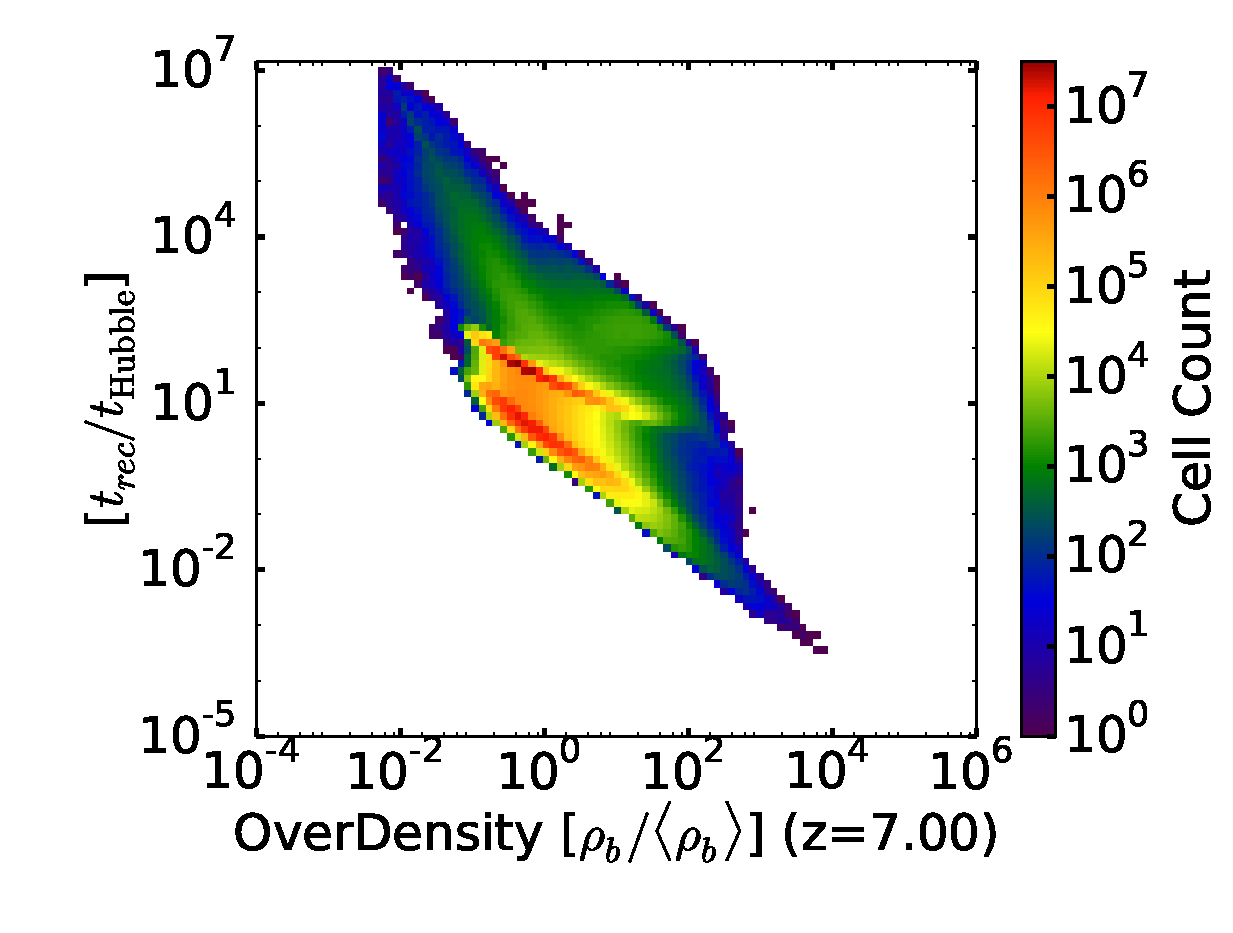
\includegraphics[trim = 5mm 8mm 0mm 0mm, clip, width=1.0\textwidth]{2_3_HD7900OverDensityRecombHubbleTime.eps}
    \end{minipage}
\\
     \begin{minipage}[h]{0.33\linewidth}
        \centering
        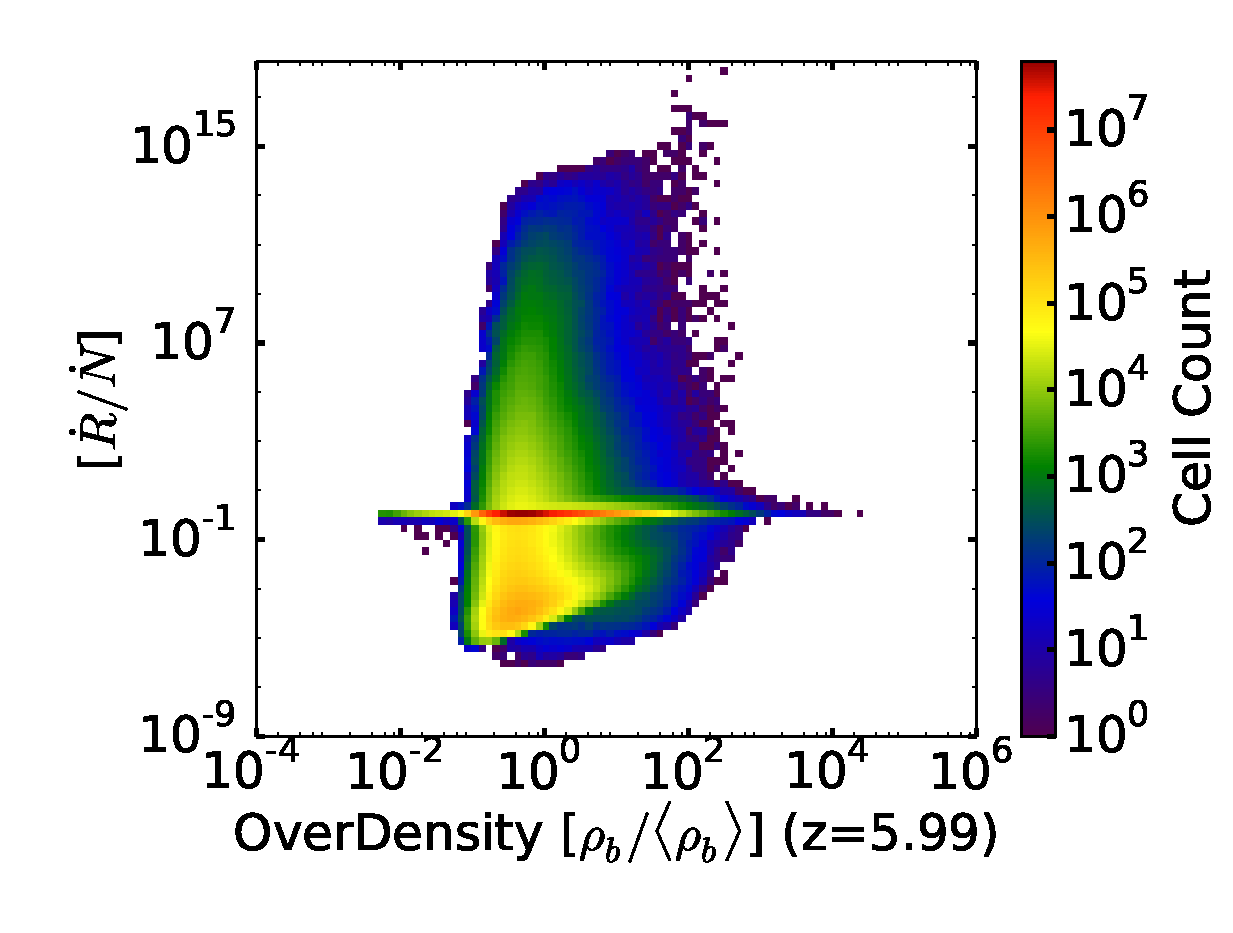
\includegraphics[trim = 5mm 8mm 0mm 0mm, clip, width=1.0\textwidth]{3_1_HD15100OverDensityRecombIonFrac.eps}
     \end{minipage}
\hspace*{-2.00mm}
    \begin{minipage}[h]{0.33\linewidth}
       \centering
       \includegraphics[trim = 5mm 8mm 0mm 0mm, clip, width=1.0\textwidth]{3_2_HD15100_recomb_contrib_v_OD.eps}
     \end{minipage}
\hspace*{-4.00mm}
    \begin{minipage}[h]{0.33\linewidth}
       \centering
       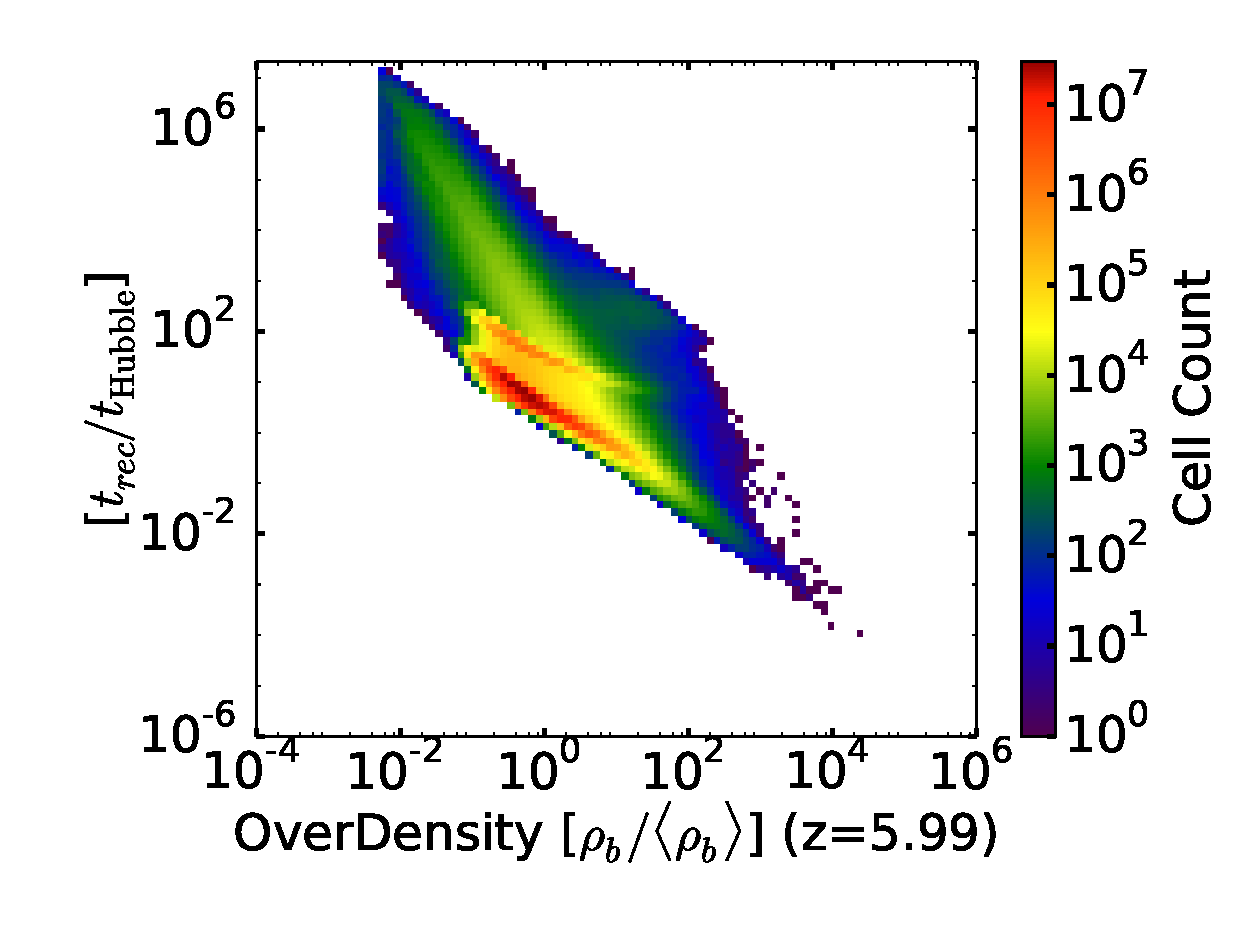
\includegraphics[trim = 5mm 8mm 0mm 0mm, clip, width=1.0\textwidth]{3_3_HD15100OverDensityRecombHubbleTime.eps}
    \end{minipage}
\\
     \begin{minipage}[h]{0.33\linewidth}
        \centering
        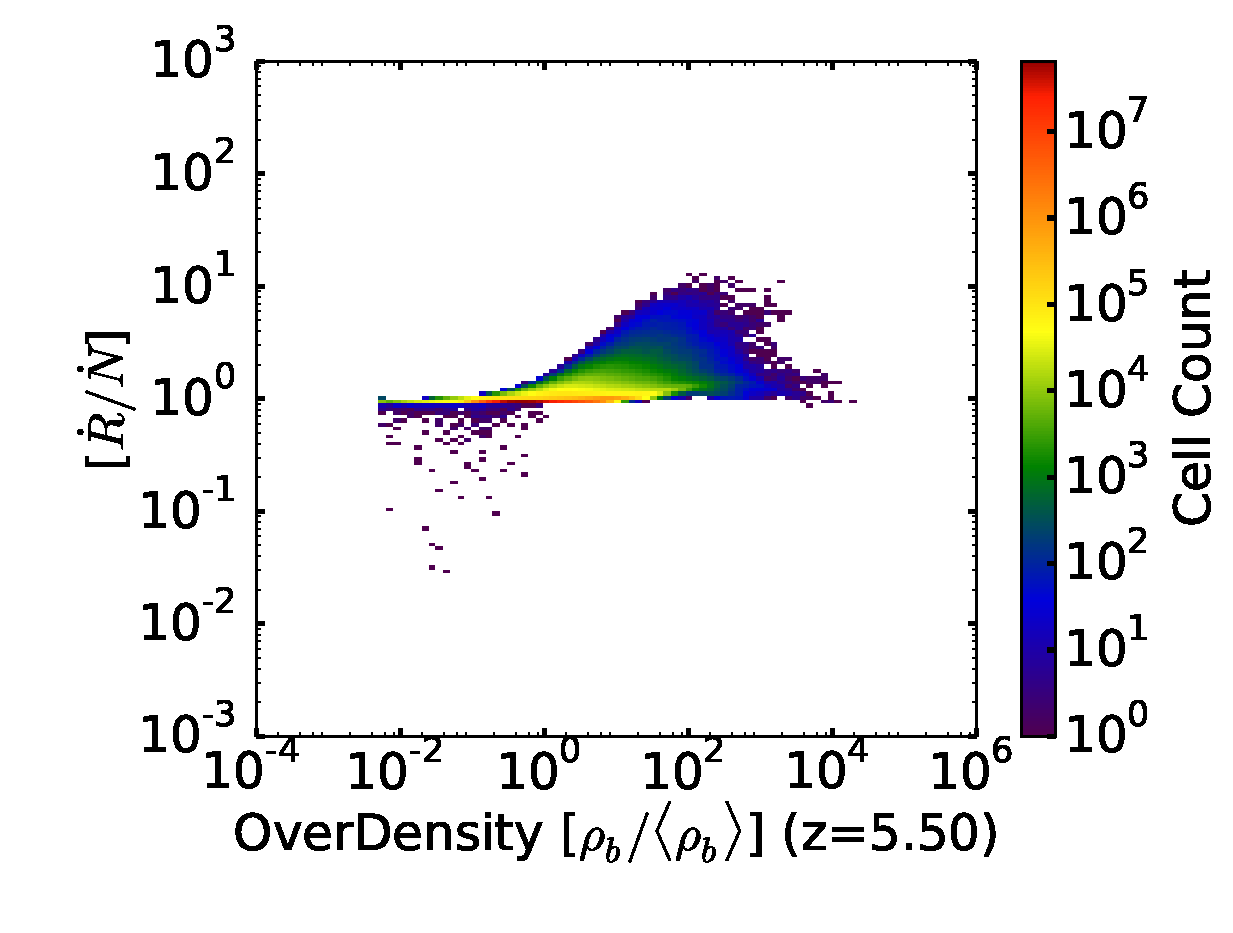
\includegraphics[trim = 5mm 8mm 0mm 0mm, clip, width=1.0\textwidth]{4_1_HD20125OverDensityRecombIonFrac.eps}
     \end{minipage}
\hspace*{-2.00mm}
    \begin{minipage}[h]{0.33\linewidth}
       \centering
       \includegraphics[trim = 5mm 8mm 0mm 0mm, clip, width=1.0\textwidth]{4_2_HD20125_recomb_contrib_v_OD.eps}
     \end{minipage}
\hspace*{-4.00mm}
    \begin{minipage}[h]{0.33\linewidth}
       \centering
       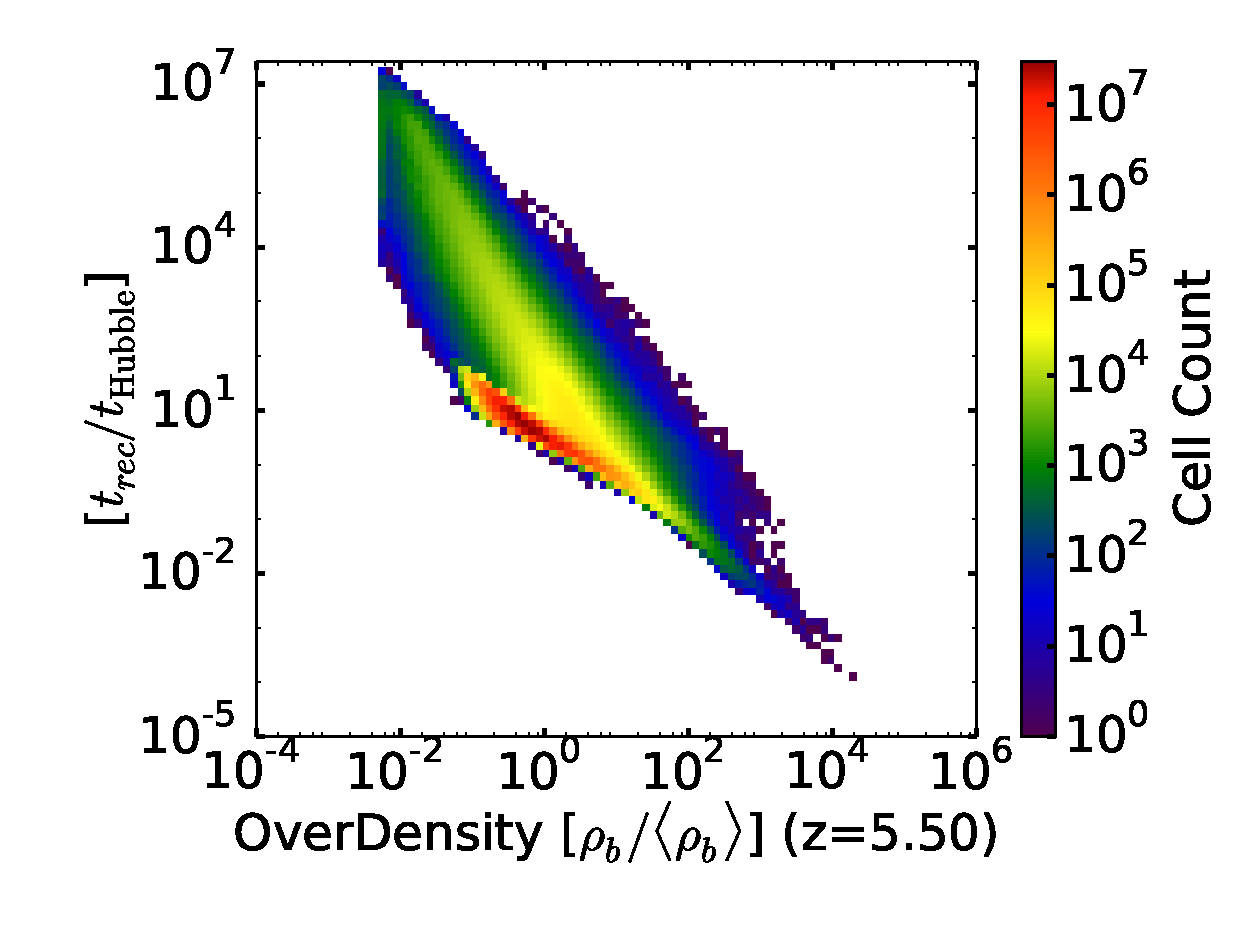
\includegraphics[trim = 5mm 8mm 0mm 0mm, clip, width=1.0\textwidth]{4_3_HD20125OverDensityRecombHubbleTime.eps}
    \end{minipage}
\\ 
     \begin{minipage}[h]{0.33\linewidth}
        \centering
        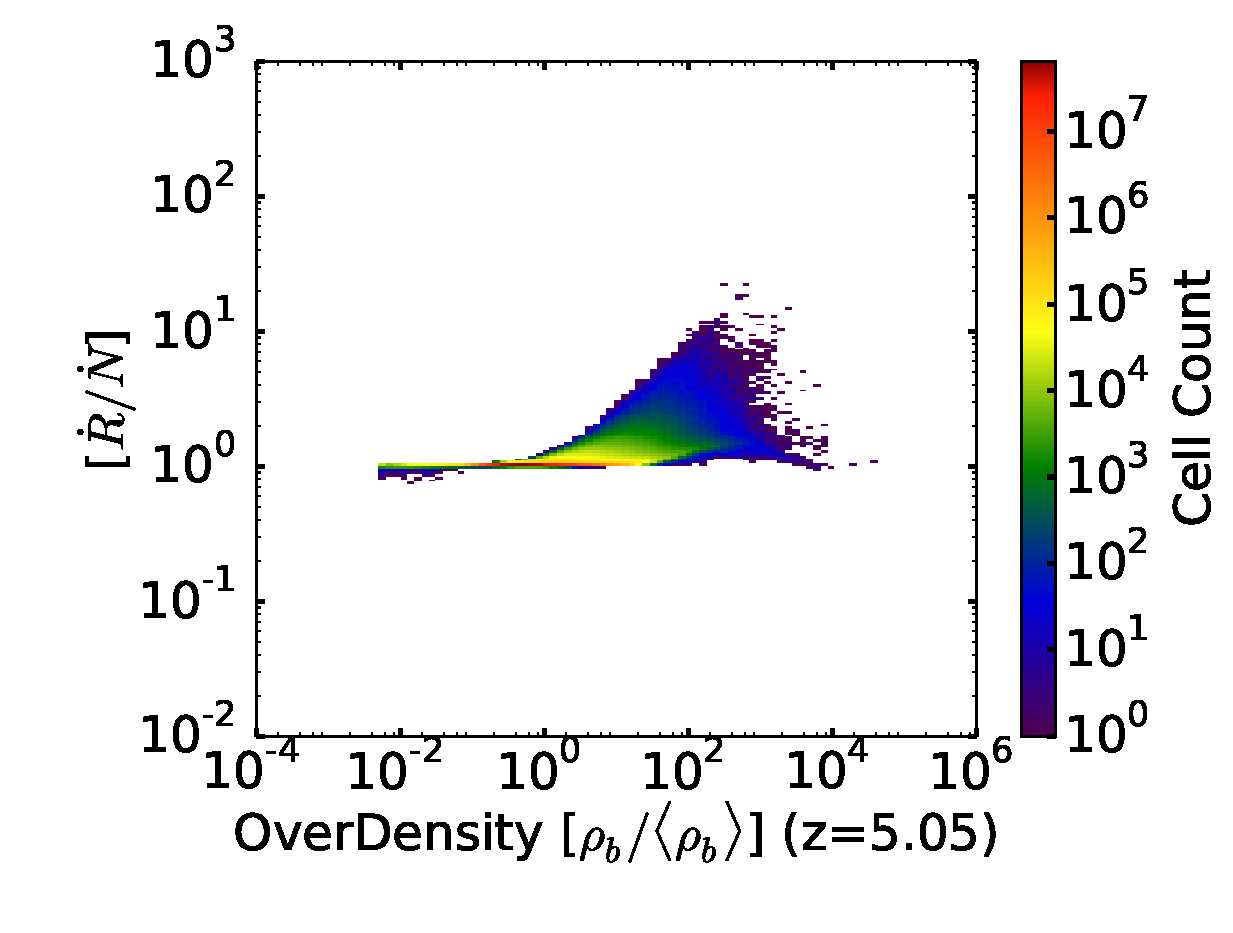
\includegraphics[trim = 5mm 8mm 0mm 0mm, clip, width=1.0\textwidth]{5_1_HD24175OverDensityRecombIonFrac.eps}
     \end{minipage}
\hspace*{-2.00mm}
    \begin{minipage}[h]{0.33\linewidth}
       \centering
       \includegraphics[trim = 5mm 8mm 0mm 0mm, clip, width=1.0\textwidth]{5_2_HD24175_recomb_contrib_v_OD.eps}
     \end{minipage}
\hspace*{-4.00mm}
    \begin{minipage}[h]{0.33\linewidth}
       \centering
       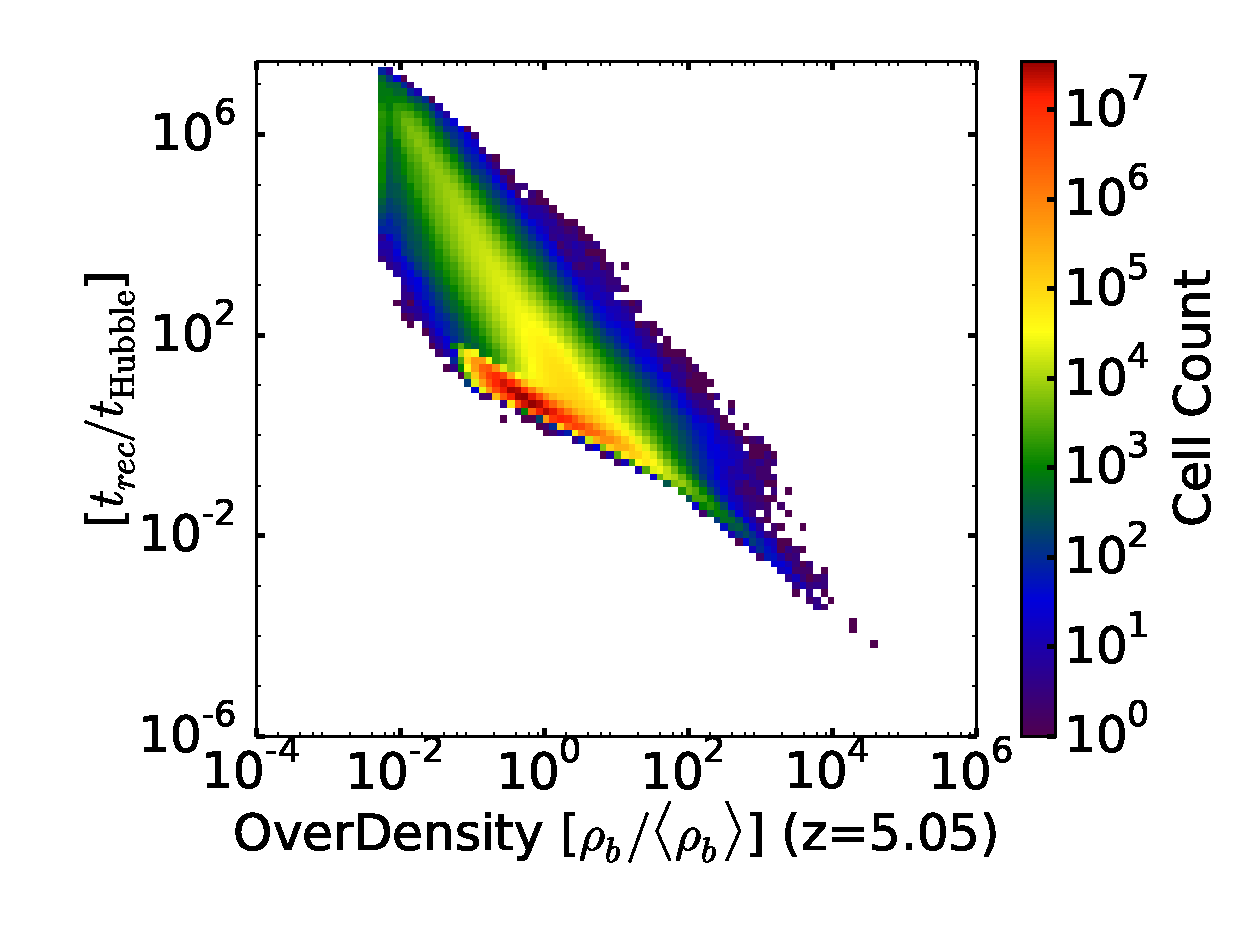
\includegraphics[trim = 5mm 8mm 0mm 0mm, clip, width=1.0\textwidth]{5_3_HD24175OverDensityRecombHubbleTime.eps}
    \end{minipage}
\\ 
    \caption{Quantifying recombination information.  Left column is a 2D distribution of recombination rate density divided by ionization rate density versus overdensity.  Middle column is plot relative bin contribution to the total recombination rate density versus overdensity bins.  The lines show the cumulative of all previous bins.  Blue line is at $\Delta_b$=100, red line is at $\Delta_b$=1.  Right column is plot of recombination time divide by Hubble time versus overdensity.  All three columns evolve with decreasing redshift from top to bottom.}
    \label{recomb}
\end{figure*}

At $z\sim9$, in the left column of Figure \ref{recomb}, we see that even though there are regions of the volume that are in approximate ionization equilibrium (indicated by the horizontal distribution near 10$^0$), there is a wide distribution of cells far out of equilibrium, some even off by $\sim120$ orders of magnitude.  The middle column shows that about 37\% of all recombinations happen below a $\Delta_b$ of 100, and about 3.2\% happen below $\Delta_b$ of 1.  The phase diagram in the right column shows that there is a bimodal distribution of cells in terms of their recombination time normalized by Hubble time.  The top concentration of cells are more neutral, having long recombination times, and the lower concentration of cells are photoionized, having smaller recombination times.  The recombination time is lower for the ionized cells simply because there are more free electrons available to recombine with protons.  The blue cloud at low $\Delta_b$ and high $t_{rec}/t_\mathrm{Hubble}$ are the small number of cells that are shock heated to $T >$10$^6$K by supernova feedback.  Due to this high temperature, even though there are more free electrons their recombination times remain long.  

At $z\sim7$, more of the volume has reached the Well Ionized level, and we see the size of the out of equilibrium distribution shrink in the left column.  Now the maximum is only $\sim37$ orders of magnitude higher compared to equilibrium.  The middle column shows about 40\% of total recombinations are happening below $\Delta_b$ of 100, and about 4.2\% happens below $\Delta_b$ of 1.  In the right column, we see roughly equal numbers of cells in the upper (more neutral) distribution as compared to the lower (more ionized) distribution, whereas the top was much greater in numbers before.  As more cells become ionized to a high degree, their recombination time will decrease and their cell counts will shift to the lower distribution.

At $z\sim6$, looking at the left column, most of the cells are now in equilibrium.  This is indicated by the peak of the distribution in red, being near zero on the y-axis.  The maximum of the distribution is now less than 19 orders of magnitude apart from equilibrium.  The middle column showing 30\% to 3.8\% recombinations below $\Delta_b$ of 100 and 1, respectively.  The right column shows that the majority of the cells are now in the more ionized distribution and have a low recombination time.  This can be verified by looking at the same redshift in Figure \ref{NeutralPhase}, where most of the cells are at the Well Ionized level compared to fewer before.

At $z\sim5.5$, after the entire volume has become Well Ionized, and the vertical spread of the distribution has collapsed to about an order of magnitude away from equilibrium with the vast majority of the cells in equilibrium.  The fraction of recombinations are 25\% and 4\% below $\Delta_b$ of 100 and 1, respectively.  Looking at the recombination time to Hubble time, we no longer see the bimodal distribution of neutral cells and highly ionized cells, we only see the bottom distribution of highly ionized cells now.  The small distribution of shock heated gas is still present, but now seem more prominent with the absence of the neutral distribution.

%{\bf added revision and subsequent concluding paragraph, please check} 
At $z\sim5$, on the left column, the few cells that are in the low density void, which were recombining slower than ionizing are now all near equilibrium.  Cells that are higher in $\Delta_b$ are more likely to be above equilibrium.  In the middle column, we see the fraction of recombinations are 16\% and 2.9\% for region below $\Delta_b$ of 100 and 1, respectively.  Not much has  changed in the recombination time column except there are fewer cells above the $\Delta_b$ of 10$^4$, possibly due to effect of Jeans smoothing.

We see that there is no real one-to-one correspondence between overdensity and the quantities we show on the y-axis.  That is because in a given panel, we are only seeing two dimensions of a multidimensional physical process that depends on locality to sources of radiation, the behavior of said sources at a given moment, the local density of neutral and ionized gas, temperature, among others.  It is helpful to speak about the average behavior in any given overdensity as we have done, but we should always keep in mind that the average may not be as representative of the wider distribution as we may think.

%\subsubsection{Thresholded Values}
%\label{ThresholdedValues}
\subsection{Investigating Thresholded Clumping Factor Analyses}
\subsubsection{Excluding Halos}
\label{ExcludingHalos}

We saw in \S\ref{Madau} that using the unthresholded H {\footnotesize II} density field to calculate $C$ via Equation \eqref{eq:clumpingfactor} yields a reasonably good estimate of when reionization completes (Figure \ref{unthresholded}). This is perhaps not surprising since we count every ionizing photon emitted and every recombination to the accuracy of Equation \eqref{eq:updatedNdot}. Possible sources of disagreement between theory and simulation are: (1) inaccuracies in estimating the recombination rate density using Equation \eqref{eq:updatedNdot}; (2) breakdown of the ``instantaneous approximation'' used to derive Equation \eqref{eq:updatedNdot} due to history-dependent effects; (3) finite propagation time for I-fronts to cross voids; and (4) numerical inaccuracies. Regarding possibility (4) we note that our mathematical formalism is photon conserving, and that our I-front tests in Paper I show that I-fronts propagate at the correct speed, which is an indication that numerical photon conservation is good. 

To investigate whether improved estimates of the recombination rate density will improve the agreement, we follow the practice of some recent investigators \citep{PawlikEtAl2009, RaicevicTheuns2011} and threshold out dense gas bound to halos, leaving only the diffuse IGM to consider. The motivation for this is that since we are only interested in the photon budget required to maintain the diffuse IGM in an ionized state, by excluding the complicated astrophysics within halos we have a simpler problem to model and resolve numerically. 

%We wondered, as the people that apply thresholding in calculating the clumping factor, what would change if the same thresholding is applied to Figure \ref{unthresholded}?  
To proceed we must calculate the ionization and recombination rate densities outside of collapsed objects. We estimate the number of ionizing photons escaping halos by multiplying  $\dot{N}_{sim}(z)$ by a global escape fraction $\bar{f}_{esc}(z)$ derived in \S\ref{escape} and plotted in Figure \ref{RadEscFraction}:
\begin{equation}
	\dot{N}_{IGM}(z)=\bar{f}_{esc}(z)\dot{N}_{sim}(z)
	\label{eq:ndot_igm}
\end{equation}
\noindent
The recombination rate density outside of halos is calculated using Equation \eqref{eq:updatedNdot} where now the clumping factor is thresholded such that only cells for which $\Delta_b < 100$ contribute to the sum. As in Figure \ref{unthresholded} we plot three curves for the recombination rate density calculated using Equation \eqref{eq:updatedNdot} using H {\footnotesize II}, baryons, and dark matter density fields. These are plotted in Figure \ref{thresholded} as green, red, and black curves, respectively. We see that the recombination rate density based on the singly thresholded H {\footnotesize II} (labeled $\dot{R}_\mathrm{tH\,II}$) and on the thresholded dark matter (labeled $\dot{R}_\mathrm{tdm}$) curve cross the ionizing emissivity curve labeled ``$\dot{N}_\mathrm{IGM}$'' at $z \approx 6.7$ in Figure \ref{thresholded}, whereas the thresholded baryon density curve (labeled $\dot{R}_{tb}$) crosses ``$\dot{N}_\mathrm{IGM}$'' at $z \sim 7.2$. Taking the doubly-thresholded H {\footnotesize II} curve as the best estimate for the recombination rate density, we find that restricting the analysis to only IGM gas yields poorer agreement than the simpler, global model of Madau, which at first blush is a perplexing result. By thresholding out the gas in galaxies we have isolated the thing we care about: the ionization balance of the IGM. Why then should the implied redshift of reionization completion become worse compared to the analysis in \S\ref{Madau}? We defer addressing this question until later sections. 

%. we plot the fraction of ionization rate density in the simulation that happens at $\Delta_b<100$ region (outside of collapsed, self shielded region) as the curve ``tIon'' in Figure \ref{EscFraction} (we will discuss Figure \ref{EscFraction} in more detail in \S\ref{ConsistencyCheck}).  This redshift dependent curve ``tIon'', we refer to as our escape fraction.  Second, we take the original ``FromSim'' curve from Figure \ref{unthresholded}, which describes the total amount of ionizing photon production rate density, and we multiply that by the escape fraction curve, the result is ``$\dot{N}_\mathrm{IGM}$'' curve in Figure \ref{thresholded}.  We calculate the ionization escape fraction using the same methodology as the recombination fraction (the same way as blue line values in the middle column of Figure \ref{recomb}).

\begin{figure}
	\includegraphics[width=0.5\textwidth]{thresholded.eps}
%	\includegraphics[width=0.5\textwidth]{threshclumping.eps}
	\caption{Same quantities as Figure \ref{unthresholded}, except now the ``$\dot{N}_\mathrm{IGM}$'' curve is the number of ionizing photons which escape into the IGM (see \S\ref{escape}). The recombination rate densities with a subscript that begins with ``t" are calculated as described in the caption for Figure \ref{unthresholded}, except that the clumping factors are computed excluding regions satisfying $\Delta_b > 100$. The curve labelled $\dot{R}_{ttHII}$ is calculated from Equation (22) using the doubly-thresholded clumping factor $C_{ttHII}$ defined in Figure \ref{threshclumping}.}
	\label{thresholded}
\end{figure}

\begin{figure}
	\includegraphics[width=0.5\textwidth]{threshclumping.eps}
	\caption{Thresholded clumping factors used in Fig. \ref{thresholded}. $C_{tHII}, C_{tb}, C_{tdm}$ are calculated using thresholded H II, baryon, and dark matter density fields, respectively, where only cells satisfying $\Delta_b < 100$ contribute. $C_{ttHII}$ is calculated from the H II density where only cells satisfying $\Delta_b < 100$ and $f_i > 0.1$ contribute.}
	\label{threshclumping}
\end{figure}

Finally, we ask how many ionizing photons per H atom are required to convert the neutral gas residing outside halos to a well ionized state. We repeat the analysis of Figure \ref{unthreshphotonbudget} and show the result in Figure \ref{threshphotonbudget}.  We see that the effect of counting only escaped photons on the photon budget is significant.  Previously, we summed $\dot{N}_{sim}(z)$ and divided by the total number of hydrogen atoms in the simulation volume, and used that as our progress variable. 
%Now we multiply the photon production by the rate escape fraction toon each time interval, to consider only the photons escaped, and divide by the number of hydrogen atoms in the simulation.  
In Figure \ref{threshphotonbudget} we sum $\dot{N}_{IGM}(z)$ and divide by the number of hydrogen atoms in the thresholded volume, and use that as our progress variable. 
Instead of needing $\sim$4 to ionize the IGM, now we only need $\sim$2 photons per hydrogen atom for 99.9\% of the universe to reach Well Ionized level. This result supports the ``photon starved'' reionization scenario discussed by \cite{BoltonHaehnelt2007}.  

%\begin{figure}
%	\includegraphics[width=0.5\textwidth]{EscFractionFit.eps}
%	\caption{}
%	\label{}
%\end{figure}

\begin{figure}
	\includegraphics[width=0.5\textwidth]{thresh_photon_per_H.eps}
	\caption{Ionized volume fraction as a function of the number of ionizing photons emitted per H atom averaged over the entire simulation volume (excluding gas inside halos) for three different ionization levels: $f_i \geq 0.1$ (blue line);  $f_i \geq 0.999$ (green line); $f_i \geq 0.99999$ (red line). Compare with Fig. \ref{unthreshphotonbudget} which includes gas inside halos.}
	\label{threshphotonbudget}
\end{figure}

%\subsubsection{Restricting Methods}
%\label{RestrictingMethods}
\subsubsection{Including Temperature Corrections}
\label{IncludingTemperatureCorrections}

During the preparation of this paper, a new way of estimating the recombinations in the IGM appeared in the literature.  The authors \citep{ShullEtAl2012,FinlatorEtAl2012} reformulated the expression for the clumping factor taking the temperature dependence of the recombination rate into account. We briefly investigate their methods here.  In order for the calculation of the clumping factor to take only IGM gas that is ionized but recombining, several additional thresholds were applied.  Equation (15) in \cite{ShullEtAl2012} is a new expression for the clumping factor, similar in form to \cite{Gnedin2000},
\begin{equation}
	C_\mathrm{RR}=\frac{\langle n_e n_\mathrm{H\,II}\alpha_B(T) \rangle}{\langle n_e \rangle \langle n_\mathrm{H\,II} \rangle \langle \alpha_B(T) \rangle}
	\label{eq:CRR}
\end{equation}
with the following thresholds applied: 1$<\Delta_b<$100, 300K$<$$T$$<10^5$K, Z$<10^{-6}$Z$_\odot$, $x_e$$>$0.05.  Here,  Z is metalicity and $x_e$ is the ionized fraction.  The reason that a lower limit threshold is applied to the baryon overdensity, the authors argued, is because very little recombinations happen there, due to the low density.  \cite{ShullEtAl2012} also provide a new formulation for ionizing photon rate density that uses this definition of the clumping factor, in their Equation (10),
\begin{align}
	\frac{dN}{dt}=4.6\times 10^{50}\mathrm{s}^{-1}\mathrm{Mpc}^{-3}\notag\\
\times \(\frac{(1+z)}{8}\)^3 T_4^{-0.845}\(\frac{C}{3}\)
	\label{eq:ShullNdot}
\end{align}
Here, T$_4$ is mean IGM temperature measured in units of 10$^4$K.  

Equation \eqref{eq:ShullNdot} is proposed as an improvement over Equation \eqref{eq:ndot}. To see if this is the case we used our data to evaluate the clumping factor C$_\mathrm{RR}$ and then used Equation \eqref{eq:ShullNdot} to calculate ionizing photon rate density versus redshift needed to maintain an ionized IGM. The result is shown in Figure \ref{Shull}. The curve labeled $\dot{R}_\mathrm{RR,T4}$ in green uses the average temperature, in units of 10$^4$K, of the region that satisfies the C$_\mathrm{RR}$ thresholds for T$_4$ in Equation \eqref{eq:ShullNdot}.  The curve $\dot{R}_\mathrm{RR}$ uses 1 in place of T$_4$ in Equation \eqref{eq:ShullNdot}, essentially fixing the IGM temperature to a constant 10$^4$K.  The green curve is lower than the red curve because the average temperature in the simulation is higher than $10^4$K. The blue curve labeled $\dot{N}_{IGM}$  is as defined previously. We see that Equation \eqref{eq:ShullNdot} predicts that reionization completes at significantly higher redshifts than exhibited by the simulation, calling into question the validity of the analysis. 

We find it curious that as the clumping factor analysis is refined through physically well-motivated modifications, it yields predictions for the redshift of reionization completion that become worse and worse, moving to higher redshift rather than lower redshift. This suggests that there is something fundamentally wrong with the whole approach, and that the seemingly good agreement found in \S\ref{Madau} was fortuitous. One worrisome aspect about the utility of Equation \eqref{eq:ShullNdot} is that the fraction of simulation volume included in the C$_\mathrm{RR}$ thresholds is actually quite small. This is illustrated in Figure \ref{volumefracCRR}. The included volume grows from 3\% at $z=9$ to only 23\% of the simulation volume by overlap. One wonders about the validity of making global statements about reionization based on such a restricted sample of the IGM. It is also unclear how we should interpret the redshift at which lines across in Figure \ref{Shull}. Should we interpret it as the redshift below which an ionization rate given by Equation \eqref{eq:ShullNdot} can keep the whole volume ionized, or only the fraction of the volume satisfying the thresholds? If it is the former, how do we account for the time it takes for I-fronts to cross neutral voids?

At this point the reader may rightfully claim that the Madau-type analysis was never meant to predict the precise redshift for reionization completion, only the ionization rate density needed to maintain the IGM in an ionized state after reionization has completed. We would agree with that. However it is effectively being used in this way when it is applied to galaxy populations at increasingly higher redshifts $z=6-7$  (cf. \cite{FanEtAl2006, RobertsonEtAl2013}). Our investigations indicate that formulae such as Equation \eqref{eq:ndot} and \eqref{eq:ShullNdot} are not reliable estimates of when reionization completes. In \S\ref{Discussion} we examine whether they can be usefully applied at lower redshifts, as originally intended. 



 
%In Figure \ref{Shull}, we show the results of using their clumping factor definition (except we do not have metalicity field in our data, therefore, there is a slight difference in the thresholding done, but it is not expected to change our results much), with most of the thresholds are applied.  The curve ``IRRFromSim''  is taking the photon production rate (``FromSim'' in Figure \ref{unthresholded}) and multiplying it by a different ionization fraction.  This time, the ionization fraction is calculated by summing the ionization from regions that satisfy the C$_\mathrm{RR}$ thresholds (1$<\Delta_b<$100, 300K$<$$T$$<10^5$K, $x$$>$0.05), and dividing it by the total ionization in the entire simulation.  The curve ``C\_RRT4'' in green uses the average temperature, in units of 10$^4$K, of the region that satisfies the C$_\mathrm{RR}$ thresholds for T$_4$ in Equation \eqref{eq:ShullNdot}.  The curve ``C\_RR'' uses 1 in place of T$_4$ in Equation \eqref{eq:ShullNdot}, essentially fixing the IGM temperature to a constant 10$^4$K.  The use of 10$^4$K in \citep{FinlatorEtAl2012} for the denominator of C$_\mathrm{RR}$ will be discussed in \S\ref{Discussion}.

%We can see that while setting the the temperature to 10$^4$K helps get the crossing with ``IRRFromSim'' closer to our expected redshift of $\sim$6, it is still further than the original or the single threshold methods.  Since this result is very sensitive on the IGM temperature, we have to beware the conclusion drawn, which we will tackle more in-depth in \S\ref{Discussion} of the article.

\begin{figure}
	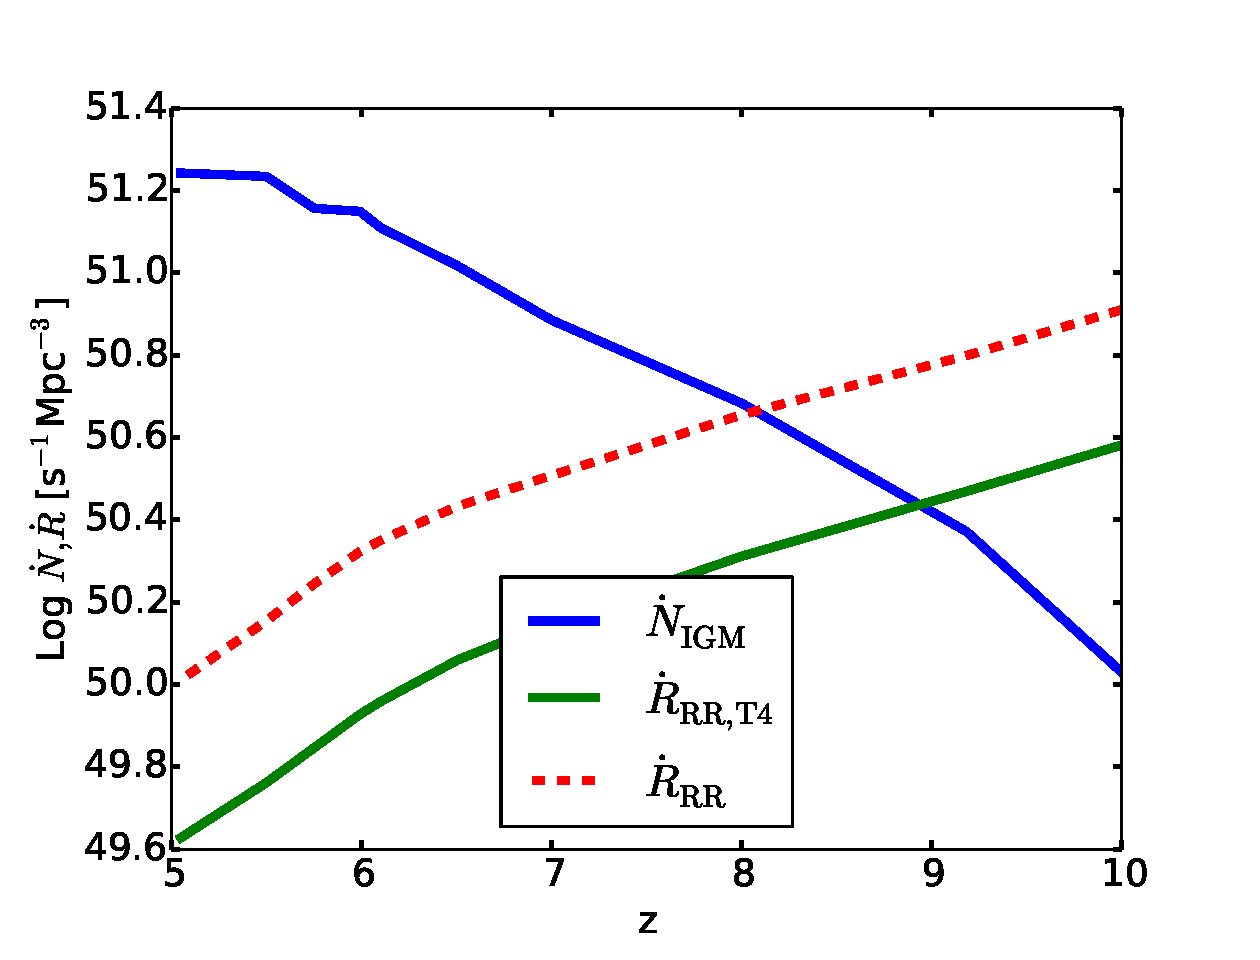
\includegraphics[width=0.5\textwidth]{Shull_thresholded.eps}
	\caption{Ionizing photon injection rate density in the IGM from the simulation $\dot{N}_{IGM}$ versus the predictions of Equation \eqref{eq:ShullNdot}, evaluated with two choices for the clumping factor which take temperature corrections into account.   The curve labeled ``$\dot{R}_\mathrm{RR,T4}$'' is from Equation \eqref{eq:ShullNdot}, with T$_4$ being the average temperature in C$_\mathrm{RR}$ region in units of 10$^4$K.  The curve ``$\dot{R}_\mathrm{RR}$'' is calculated the same way as $\dot{R}_\mathrm{RR,T4}$ except now T$_4$ is set to 1 in Equation \eqref{eq:ShullNdot}, for an effective IGM temperature of 10$^4$K.}
	\label{Shull}
\end{figure}

\begin{figure}
	\includegraphics[width=0.5\textwidth]{volumefracCRR.eps}
	\caption{Evolution of the volume filling fraction with redshift of regions satisfying the C$_\mathrm{RR}$ thresholding criteria.}
	\label{volumefracCRR}
\end{figure}

\subsection{Comparing Clumping Factors}
\label{ClumpingFactorEvolution}

For ease of comparison we collect into one plot all the H {\footnotesize II} clumping factors used in the previous sections. The unthresholded H {\footnotesize II} calculated using Equation \eqref{eq:clumpingfactor} is denoted C$_\mathrm{H\,II}$. The singly thresholded clumping factor is denoted C$_\mathrm{tH\,II}$, in which the threshold $\Delta_b<100$ is being applied. The curve labeled C$_\mathrm{RR}$ plots the evolution of Equation \eqref{eq:CRR} with the following thresholds: 1$<\Delta_b<$100, 300K$<$$T$$<10^5$K, $x_e$$>$0.05. For comparison we also plot a doubly thresholded H {\footnotesize II} clumping factor denoted C$_\mathrm{ttH\,II}$ with thresholds $\Delta_b<100$ and $x_e>0.05$, which can be thought of as the clumping factor inside H {\footnotesize II} regions excluding the dense gas in halos. 
%We now show the clumping factors we calculated and used in Equation \eqref{eq:updatedNdot}, \eqref{eq:ShullNdot}.  The two equations estimate the amount of photon production rate density required to keep the universe ionized.  Figure \ref{ClumpingFactors} shows various clumping factors that is calculated using the H {\footnotesize II} field.  The first three clumping factors are calculated using Equation \eqref{eq:clumpingfactor} with H {\footnotesize II} number density.  The prefix ``t'' indicates the threshold of $\Delta_b<100$ being applied.  The ``tt'' prefix indicates two thresholds are applied, they are: $1<\Delta_b$ and $x>0.05$.  The curve ``ttC$_\mathrm{H\,II}$'' is not used in our other analysis, we show it here only to illustrate the effects of applying different thresholds.  The last curve is the C$_\mathrm{RR}$ clumping factor from Equation \eqref{eq:CRR} with the following thresholds: 1$<\Delta_b<$100, 300K$<$$T$$<10^5$K, $x$$>$0.05.

We see a clear trend that as more thresholds are applied the lower the value of the clumping factor goes.  This is because as more regions of the volume are excluded from the averaging process the remaining regions are more homogeneous exhibiting less variations.  If no thresholds are applied, the H {\footnotesize II} clumping factor starts around 200 at $z\sim9$ (Figure \ref{unthresholded}).  Such high values arise because when the first couple of ionizing sources created high H {\footnotesize II}, they are localized and spread far apart, making the H {\footnotesize II} density very clumpy.  As more of the universe is ionized, the H {\footnotesize II} density becomes more homogeneous.  We see the single and double thresholded H {\footnotesize II} clumping factors become the same after overlap with a value of $\sim 4.5$  because the second threshold $x_e>0.05$ is satisfied everywhere. 

The clumping factor that is not based on the H {\footnotesize II} density alone is C$_\mathrm{RR}$.  We see from Equation \eqref{eq:CRR}, C$_\mathrm{RR}$ depends on electron number density, H {\footnotesize II} number density, and the case B hydrogen recombinationation coefficient $\alpha_B(T)$, which is itself dependent on the gas temperature T (fit to Table 2.7 in \cite{OsterbrockFerland2006} implemented in Enzo).  $\alpha_B(T)$ depends on T to a negative power and this causes Equation \eqref{eq:CRR} to sometimes have a very low numerator compared to the denominator.  This as well as the exclusion of gas in the voids leads to the low clumping factor value of $\sim 2$ we see in the graph.  It is very possible to have a value that is smaller than unity, which can lead to even more confusion with the original definition of the clumping factor in Equation \eqref{eq:clumpingfactor}.  There, the clumping factor can only have a value of greater than 1, and 1 occurs only in the case of homogeneous distribution of the gas number density.

\begin{figure}
	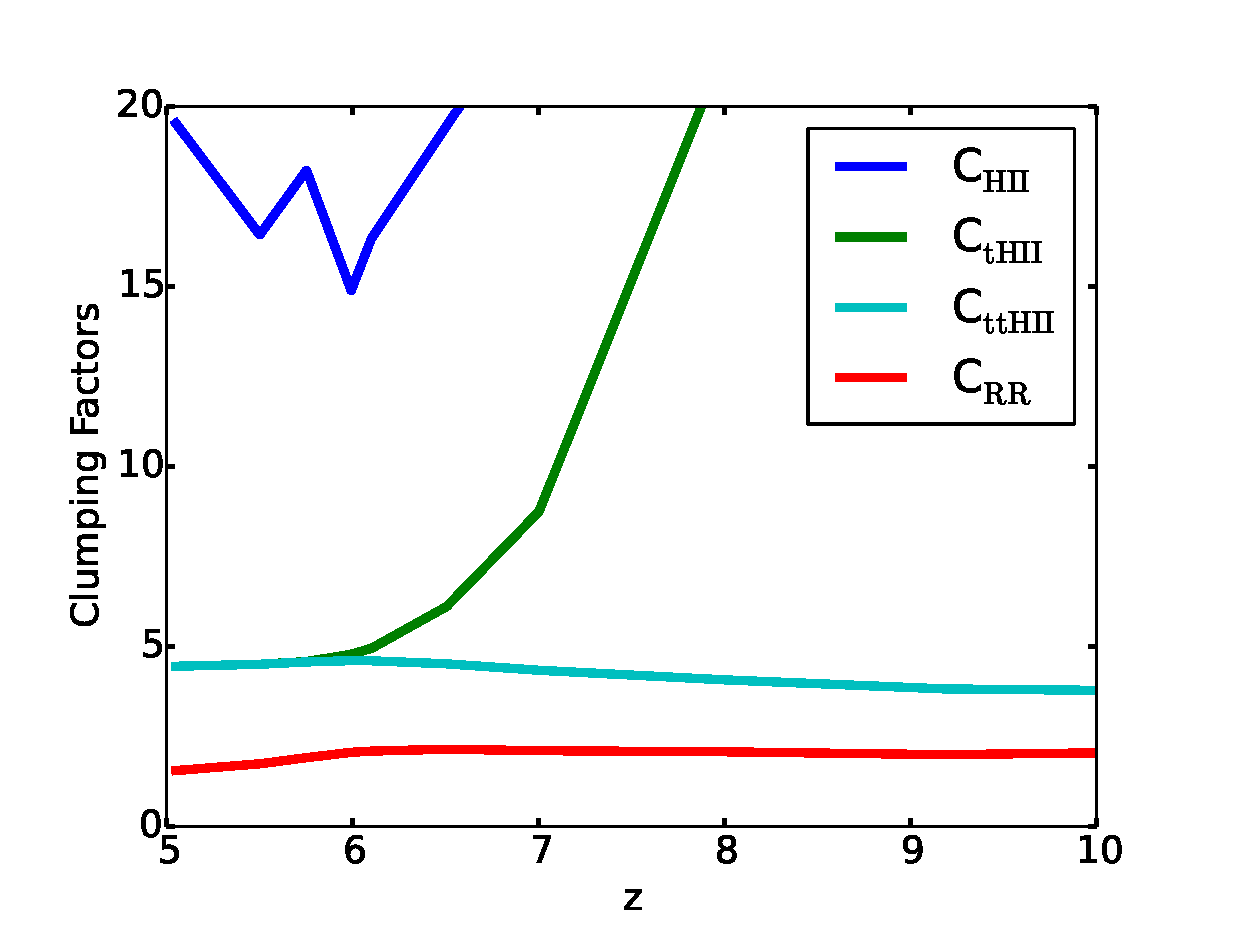
\includegraphics[width=0.5\textwidth]{ClumpingFactors.eps}
	\caption{Various clumping factors versus redshift.  C$_\mathrm{H\,II}$ is Equation \eqref{eq:clumpingfactor} used in $\dot{R}_\mathrm{H\,II}$ curve in Figure \ref{unthresholded}, C$_\mathrm{tH\,II}$ is used in $\dot{R}_\mathrm{tH\,II}$ curve in Figure \ref{thresholded}, C$_\mathrm{ttH\,II}$ is clumping factor with two thresholds applied, $\Delta_b < 100$ and $f_i>0.1$, shown here solely for comparison.  C$_\mathrm{RR}$ is the value of recombination rate clumping factor from Equation \eqref{eq:CRR} with the 5 thresholds applied.}
	\label{ClumpingFactors}
\end{figure}

